\documentclass[border=8pt]{standalone}
\usepackage{tikz}
\usetikzlibrary{positioning, arrows.meta, calc}
\usepackage[T1]{fontenc}
\usepackage{lmodern}

\definecolor{ax1}{RGB}{109, 40, 217}    % purple — Ontology
\definecolor{ax2}{RGB}{37, 99, 235}     % blue — Identity
\definecolor{ax3}{RGB}{13, 148, 136}    % teal — Evidence
\definecolor{ax4}{RGB}{217, 119, 6}     % amber — Formalism
\definecolor{ax5}{RGB}{225, 29, 72}     % rose — Target
\definecolor{txtdark}{RGB}{30, 41, 59}
\definecolor{txtsub}{RGB}{71, 85, 105}
\definecolor{txtmuted}{RGB}{100, 116, 139}
\definecolor{conn}{RGB}{203, 213, 225}

\begin{document}
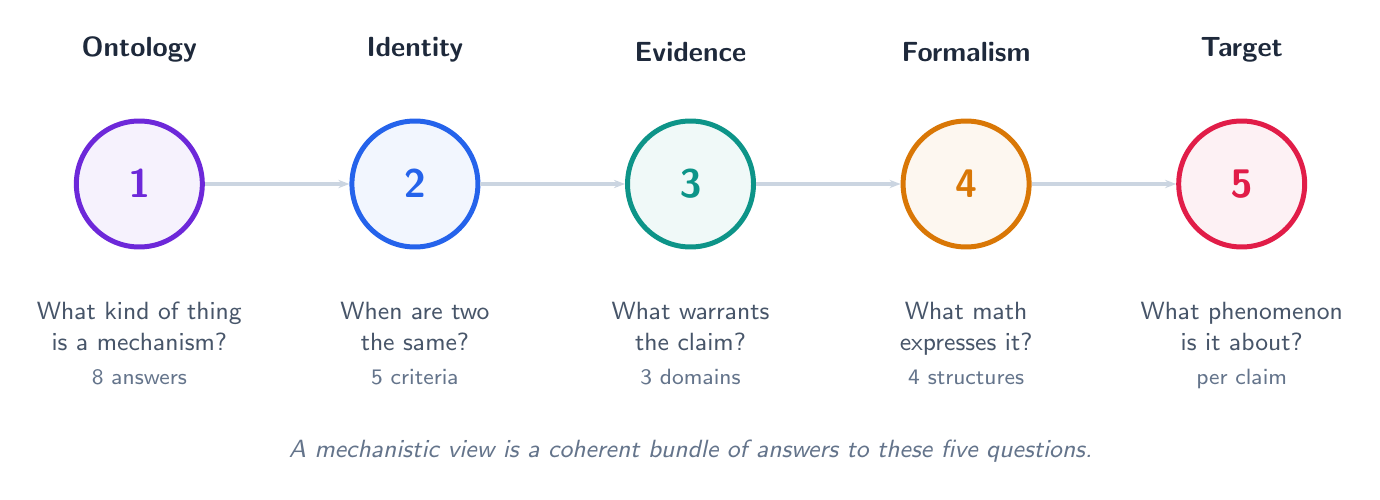
\begin{tikzpicture}[
  every node/.style={font=\sffamily},
  circ/.style 2 args={
    circle, draw=#1, line width=1.8pt, fill=#1!6,
    minimum size=1.6cm, inner sep=0pt,
  },
  cnum/.style={font=\sffamily\Large\bfseries},
  ctitle/.style={font=\sffamily\bfseries, text=txtdark},
  cq/.style={font=\sffamily\small, text=txtsub, align=center},
  ccount/.style={font=\sffamily\footnotesize, text=txtmuted},
  arr/.style={-{Stealth[length=4pt, width=3pt]}, conn, line width=1.2pt},
]

\def\sep{3.5}

% Circles
\foreach \i/\col/\name/\qa/\qb/\cnt in {
  0/ax1/Ontology/{What kind of thing}/{is a mechanism?}/8 answers,
  1/ax2/Identity/{When are two}/{the same?}/5 criteria,
  2/ax3/Evidence/{What warrants}/{the claim?}/3 domains,
  3/ax4/Formalism/{What math}/{expresses it?}/4 structures,
  4/ax5/Target/{What phenomenon}/{is it about?}/per claim%
}{
  \node[circ={\col}{}] (c\i) at (\i*\sep, 0) {};
  \node[cnum, text=\col] at (c\i) {\the\numexpr\i+1\relax};
  \node[ctitle, above=0.6cm of c\i] {\name};
  \node[cq, below=0.55cm of c\i] {\qa\\\qb};
  \node[ccount, below=1.4cm of c\i] {\cnt};
}

% Arrows
\foreach \i in {0,...,3}{
  \pgfmathtruncatemacro{\j}{\i+1}
  \draw[arr] (c\i.east) -- (c\j.west);
}

% Tagline
\node[font=\sffamily\small\itshape, text=txtmuted, below=2.3cm of c2]
  {A mechanistic view is a coherent bundle of answers to these five questions.};

\end{tikzpicture}
\end{document}
